%% ===========================================================================
%% IEEE RA-L manuscript -- DOUBLE-ANONYMOUS submission draft.
%% Build:  pdflatex main ; bibtex main ; pdflatex main ; pdflatex main
%% NOTE: This is a working draft. Items marked [AUTHOR TO PROVIDE] MUST be filled
%% before submission. Self-citations \cite{ownRobustMI2025,ownDualValidation2025}
%% must be anonymized ("[Anonymous]") for review per RA-L double-anonymous policy.
%% ===========================================================================
\documentclass[10pt,journal]{IEEEtran}
\usepackage{amsmath,amssymb,amsfonts}
\usepackage{graphicx}
\usepackage{booktabs}
\usepackage{url}
\usepackage[hidelinks]{hyperref}
\usepackage{xcolor}
\newcommand{\todo}[1]{\textcolor{red}{\textbf{[#1]}}}
\graphicspath{{figures/}}

\begin{document}

\title{Decision-Point Shared Control for Self-Calibrating\\ Motor-Imagery BCI Navigation of a Mobile Robot}

\author{Anonymous Author(s)\\ \textit{Paper submitted for double-anonymous review}%
\thanks{This work was conducted under an approved institutional review board (IRB) protocol.}}

\markboth{IEEE Robotics and Automation Letters. Preprint version.}%
{Anonymous \MakeLowercase{\textit{et al.}}: Decision-Point Shared Control for Motor-Imagery BCI Navigation}

\maketitle

\begin{abstract}
Motor-imagery (MI) brain--computer interfaces (BCIs) are attractive for hands-free
robot control but are limited by noisy, non-stationary electroencephalography (EEG):
decoders trained offline degrade across sessions, and most systems require per-user
training data and continuous decoding. We present a \emph{decision-point} shared-control
framework in which the BCI is queried only at navigation junctions: a mobile robot drives
autonomously along corridors and, on reaching a wall, halts and waits for a single left/right
MI command that selects the turn. The decoder is trained once and \emph{frozen}; at the start
of each session an unsupervised, label-free calibration recomputes only the covariance
alignment reference, and an adaptive \emph{boundary-recentering} rule continuously tracks the
user's neutral operating point so a fixed model stays calibrated online without retraining.
We evaluate two decoders---Euclidean-Alignment Filter-Bank CSP with shrinkage LDA, and a
Riemannian tangent-space pipeline with logistic regression---crossed with personalized (per-user)
and generalized (multi-user, pooled) training, in a $2{\times}2$ in-the-loop study on four users
driving a first-person robot maze simulator. Across 16 trials the users completed every maze
(16/16), with 92.0\,\% first-attempt \emph{corner} accuracy and a median command latency of
0.20\,s. A single generalized decoder performed comparably to per-user decoders at the task
level, and because decision-point shared control renders command errors recoverable, imperfect
per-command decoding still yielded full task completion.
\end{abstract}

\begin{IEEEkeywords}
Brain--computer interface, motor imagery, shared control, mobile robot navigation, EEG,
transfer learning, human--robot interaction.
\end{IEEEkeywords}

% ============================================================ I. INTRODUCTION
\section{Introduction}
\IEEEPARstart{B}{rain}--computer interfaces (BCIs) based on motor imagery (MI) let a user
issue commands by imagining movements, offering a control channel for people with severe motor
impairment~\cite{leeb2015telepresence,tonin2021review}. Translating MI-BCIs from offline
benchmarks to live robot control, however, remains difficult for three reasons. First, EEG is
noisy and \emph{non-stationary}: a decoder trained in one session loses accuracy in the next as
electrode montage, impedance, and user state drift~\cite{ownDualValidation2025,wu2022transferreview}.
Second, most pipelines require \emph{per-user} training data, adding an enrollment burden.
Third, \emph{continuous} decoding forces the user to sustain imagery throughout operation and
exposes every window to misclassification, which for a moving robot can be unsafe.

We address these issues through the interaction design rather than through the classifier alone.
Our premise is that navigation only needs \emph{discrete} choices at \emph{decision points}
(corridor junctions); between junctions the robot can drive autonomously. This reduces the BCI's
role to one binary command per junction and lets the system reject or defer during ambiguous
intervals. We combine this with an \emph{unsupervised, label-free} online adaptation scheme that
keeps a frozen decoder calibrated to the current session without retraining.

Prior work in our line established accurate \emph{offline} MI classification and quantified the
across-session accuracy loss---the ``laboratory-to-practice'' gap~\cite{ownRobustMI2025,ownDualValidation2025}.
This paper closes that gap in a live navigation loop and evaluates it at the \emph{task} level.
Our contributions are:
\begin{enumerate}
\item A \textbf{decision-point shared-control} navigation framework that restricts BCI
involvement to junction turn-choices (about one command per corner, 0.20\,s median latency),
with autonomous heading-hold and a range-based stop between junctions (Sec.~\ref{sec:controller}).
\item An \textbf{unsupervised, label-free session-adaptation} scheme---alignment-reference
recomputation plus adaptive decision-boundary recentering---that keeps a \emph{frozen} decoder
calibrated online with no labels and no retraining (Sec.~\ref{sec:adapt}).
\item A \textbf{$2{\times}2$ in-the-loop study} (two decoders $\times$ personalized/generalized
training) evaluating both decoder families and the effect of pooling users' data, at the task
level (Sec.~\ref{sec:results}).
\item A \textbf{task-level evaluation} distinguishing per-corner from per-command accuracy and
showing that recoverable errors under shared control convert $\sim$92\,\% per-corner decoding
into 100\,\% task completion.
\end{enumerate}
We evaluate in a kinematic robot-maze \emph{simulator}; the scope and its limits are stated
explicitly in Secs.~\ref{sec:method-exp} and~\ref{sec:limits}.

% ============================================================ II. RELATED WORK
\section{Related Work}
\textbf{MI decoding.} Common Spatial Patterns (CSP)~\cite{ramoser2000csp,blankertz2008csp} and
its filter-bank extension (FBCSP)~\cite{ang2008fbcsp,ang2012fbcsp} with (shrinkage-regularized)
LDA~\cite{blankertz2011shrinkage,ledoit2004shrinkage} remain strong, data-efficient baselines.
Covariance-manifold methods classify EEG spatial covariances directly on the symmetric
positive-definite manifold via Riemannian distances and tangent-space
projection~\cite{barachant2012riemann,barachant2013tangent,congedo2017primer,yger2017review}.
Deep networks (e.g., EEGNet, deep/shallow ConvNets, transformers) are the modern
alternative~\cite{lawhern2018eegnet,schirrmeister2017deep,song2023conformer,altaheri2023atcnet,roy2019dlreview}
but are data-hungry and heavier to deploy; we adopt lightweight decoders suitable for embedded,
real-time use. EEG intent recognition for human--robot interaction on comparable acquisition
hardware has been studied offline with FB-CSP and linear
classifiers~\cite{labAssessmentHRI2024,labComparative2024}.

\textbf{Cross-session/subject transfer.} Alignment methods reduce distribution shift: Euclidean
Alignment (EA) recentres raw trials by their covariance mean~\cite{he2020ea}, while Riemannian
alignment and Procrustes analysis transport covariance distributions on the
manifold~\cite{zanini2018transfer,rodrigues2019rpa}; subject-independent deep models pursue the
same goal~\cite{kwon2020subjectindependent,wu2022transferreview}. These correct the covariance
statistics but not necessarily the classifier's operating point, which we address online.

\textbf{BCI-controlled robots.} MI and hybrid BCIs have driven wheelchairs and mobile
robots~\cite{millan2004mobilerobot,galan2008wheelchair,tsui2011selfpaced,carlson2013wheelchair,zhang2021survey},
robotic arms~\cite{meng2016robotarm,edelman2019scirobotics}, wheelchairs with automated
navigation~\cite{iturrate2009wheelchair}, and telepresence
platforms~\cite{leeb2015telepresence}, increasingly with \emph{shared control} that blends user
intent with autonomy~\cite{carlson2013wheelchair,xu2023sharedcontrol,tonin2021review}.
Asynchronous/self-paced control and command rejection avoid forcing a decision every
window~\cite{mason2000switch,tsui2011selfpaced}, and error-related potentials have been used to
detect mistakes~\cite{ferrez2008errp,chavarriaga2010errp}. Our decision-point scheme is in this
tradition but pairs discrete junction commands with an unsupervised, label-free recalibration of
a frozen decoder and reports task-level rather than only classification metrics.

% ============================================================ III. SYSTEM OVERVIEW
\section{System Overview and Problem Formulation}
The system (Fig.~\ref{fig:system}) has three parts: EEG acquisition and decoding, an
unsupervised online adaptation stage, and a decision-point robot controller communicating over a
WebSocket. EEG is acquired from an OpenBCI Cyton\,+\,Daisy stack (15 usable channels at the
10--20 sensorimotor sites, sampled at $f_s=125$\,Hz). Every stride ($\Delta t = 0.2$\,s) the most
recent 2.0\,s window is decoded, yielding a $5$\,Hz stream of tentative left/right decisions that
are smoothed and, when confident and stable, committed as a command.

\textbf{Problem.} Let $x\in\mathbb{R}^{C\times T}$ be a band-limited EEG window ($C$ channels,
$T$ samples). A frozen decoder produces a log-odds score $s = g(x)\in\mathbb{R}$ toward the
``right'' class. Because the score distribution shifts across sessions and users, a fixed
threshold on $s$ is unreliable. We seek an unsupervised, label-free mapping from $s$ to a
committed command $u\in\{\text{left},\text{right},\varnothing\}$ that (i) tracks each session's
operating point without retraining $g$, and (ii) abstains ($\varnothing$) when evidence is weak,
so that the robot acts only on reliable commands at decision points.

\begin{figure}[t]\centering
  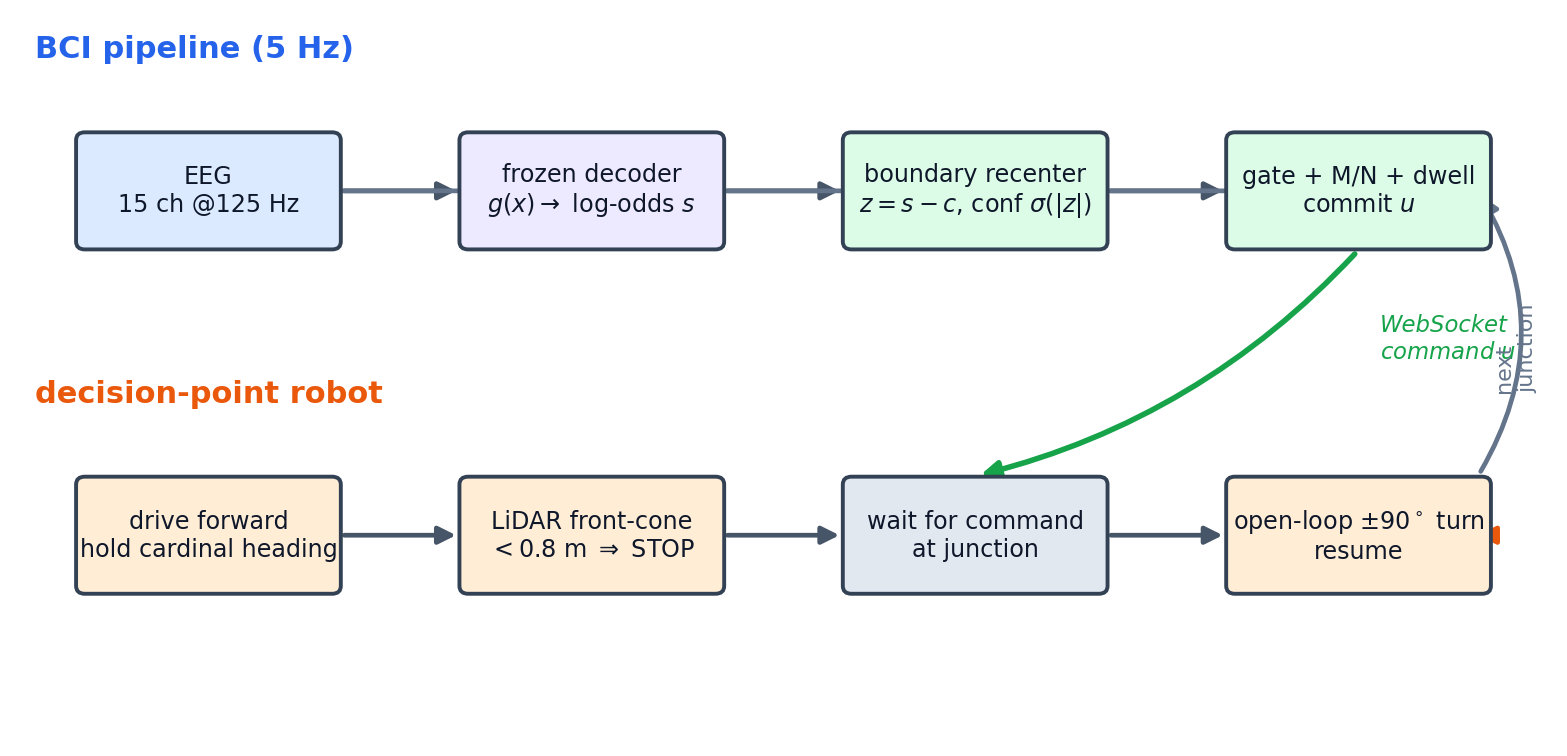
\includegraphics[width=\linewidth]{system.png}
  \caption{Decision-point shared-control loop. The frozen BCI pipeline (top) emits committed
  left/right commands at $5$\,Hz after recentering and gating; the robot (bottom) drives
  autonomously, stops at a wall, executes the commanded turn, and proceeds to the next junction.}
  \label{fig:system}
\end{figure}

% ============================================================ IV. METHOD
\section{Proposed Method}
\subsection{Decoders}
Both decoders share the interface $g:\;$window$\to$log-odds, and a filter bank of four bands
$\mathcal{B}=\{(8,12),(11,15),(14,20),(20,30)\}$\,Hz realised with causal minimum-phase FIR
filters, so decoding is real-time.

\emph{(A) EA\,+\,FB-CSP.} Per band $b$ and trial $i$, the spatial covariance is
$C_i=\tfrac{1}{T}X_iX_i^{\!\top}$ and the Euclidean-Alignment reference is the mean
$R=\tfrac{1}{N}\sum_i C_i$~\cite{he2020ea}. With $R=V\Lambda V^{\!\top}$, whitening each trial by
$R^{-1/2}=V\Lambda^{-1/2}V^{\!\top}$ makes the aligned mean covariance identity:
\begin{equation}
\tilde{X}_i = R^{-1/2}X_i,\qquad \tfrac{1}{N}\textstyle\sum_i \tilde C_i = I .
\end{equation}
CSP then extracts two components per band; the feature is their log-variance, and a
shrinkage-LDA~\cite{ledoit2004shrinkage} produces the log-odds
$s = w^{\!\top} f + b_0$.

\emph{(B) Riemannian tangent-space.} Per band, a Ledoit--Wolf covariance $C_i$ is recentred by
the Riemannian (Fr\'echet) mean $\bar C=\arg\min_M\sum_i \delta_R(M,C_i)^2$, where
$\delta_R(A,B)=\lVert\log(A^{-1/2}BA^{-1/2})\rVert_F$~\cite{barachant2012riemann,zanini2018transfer};
the recentred matrices are mapped to the tangent space at the identity,
$v_i=\mathrm{upper}(\log(\bar C^{-1/2}C_i\bar C^{-1/2}))$~\cite{barachant2013tangent}, and a
logistic regression gives $s=w^{\!\top}v+b_0$.

At deployment the model weights are \emph{frozen}. A $45$\,s calibration block recomputes only the
alignment reference ($R$ or $\bar C$) from the live session, absorbing the covariance shift
without labels.

\subsection{Unsupervised boundary recentering and gating}\label{sec:adapt}
Alignment corrects covariance statistics but not where the classifier's boundary sits, so a
session's log-odds can be offset (a neutral/rest state read as a confident class). We track the
neutral operating point online. Seeding from the calibration median $c_0=\mathrm{median}_j\,s_j$,
the recentred margin, committed side, and confidence are
\begin{align}
z_t &= s_t - c_t, &
\hat y_t &= \begin{cases}\text{right}, & z_t>0\\ \text{left}, & z_t\le 0\end{cases}, \\
\mathrm{conf}_t &= \sigma(|z_t|) = \frac{1}{1+e^{-|z_t|}} .
\end{align}
The neutral is updated only from \emph{rest-like} windows (small margin), so sustained imagery
never drags the boundary, and it is clamped near its seed:
\begin{equation}
c_{t+1}=\mathrm{clip}\!\big(c_t+\alpha(s_t-c_t),\,c_0-\Delta,\,c_0+\Delta\big)\ \text{if } |z_t|<\tau .
\end{equation}
A window is eligible to commit only if $\mathrm{conf}_t\ge\theta$; because confidence is measured
from the recentred margin, this gate is also a \emph{dead-zone} around neutral, so idle/rest does
not commit (Fig.~\ref{fig:method}). We use $\alpha=0.01$, $\Delta=2.0$, $\theta=0.85$
(Table~\ref{tab:params}).

\begin{figure}[t]\centering
  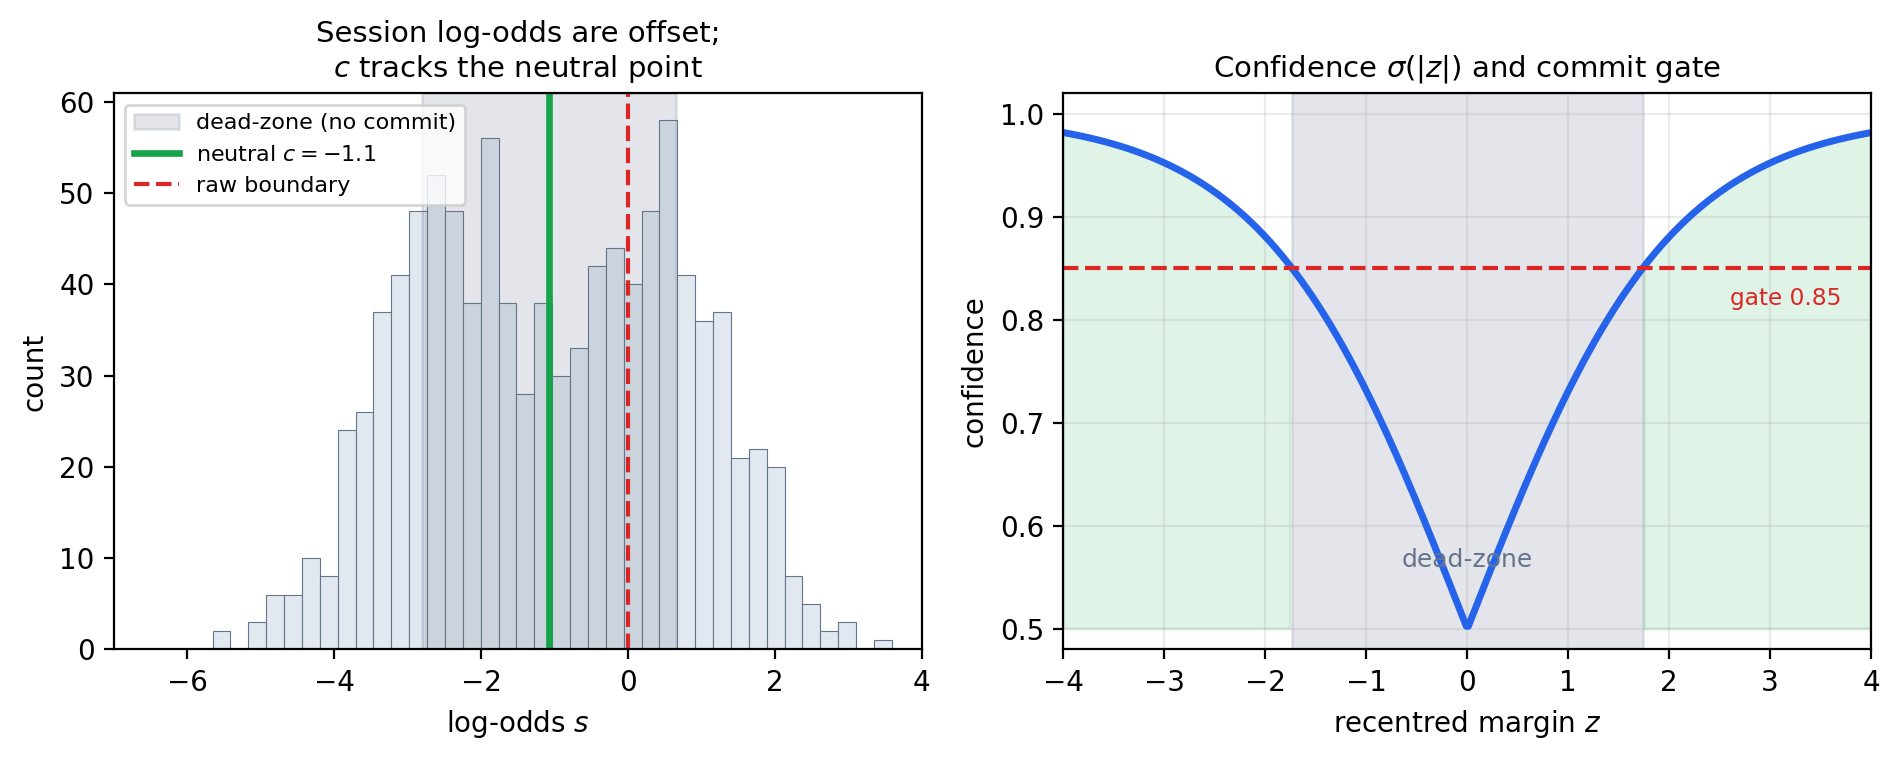
\includegraphics[width=\linewidth]{method_recenter.png}
  \caption{Unsupervised boundary recentering. Left: a session's log-odds are offset, so the
  adaptive neutral $c$ (green) sits away from the raw boundary. Right: confidence $\sigma(|z|)$
  with the commit gate; the gate forms a dead-zone around neutral so weak/rest evidence abstains.}
  \label{fig:method}
\end{figure}

\subsection{Temporal smoothing and commitment}
Gated per-window decisions feed an $M$-of-$N$ majority vote ($N{=}5$, $M{=}4$) followed by a
dwell requirement ($D{=}3$ consecutive consensus windows) before a command is committed and sent
to the robot. This tolerates isolated misclassifications while keeping commitment latency low.

\subsection{Decision-point controller}\label{sec:controller}
Between junctions the robot drives forward at constant speed while a proportional law holds the
nearest cardinal heading. A simulated planar LiDAR provides a front-cone ($\pm15^\circ$) minimum
range; when it falls below $0.8$\,m the robot stops and enters a waiting state at the decision
point. It remains stopped until a committed BCI command arrives, then executes an open-loop
$\pm90^\circ$ turn about the snapped cardinal heading (which prevents heading drift from
accumulating) and resumes. If the turn is wrong the robot faces a wall, re-stops, and waits
again---so an error is locally \emph{recoverable} at the cost of additional commands, never a
crash or an off-course excursion.

% ============================================================ V. METHODOLOGY
\section{Experimental Methodology}\label{sec:method-exp}
\textbf{Simulation scope.} Experiments use a first-person robot-maze simulator with a
TIAGo/PMB2-shaped robot. The simulator integrates a kinematic unicycle pose at a fixed timestep
and models collisions geometrically; it is \emph{not} a physics/dynamics engine, and autonomy is
limited to heading-hold and range-based stopping. It provides a controlled, repeatable test of
the BCI--shared-control loop; physical-robot validation is future work (Sec.~\ref{sec:limits}).

\textbf{Data and decoders.} Offline MI data were collected from eight participants under an
approved IRB protocol, each contributing several sessions of cued left/right-hand imagery (one
further participant was excluded for signal-quality reasons). Personalized decoders are trained
on the driving user's own data; generalized decoders are trained on the pooled data of all eight
participants \emph{including} the driving user (i.e., a single shared multi-user model, not a
subject-held-out model).

\textbf{Task and design.} Each trial navigates a procedurally generated 40-corner maze. We use a
$2{\times}2$ design---decoder $\{$EA+FB-CSP, Riemannian-TS+LR$\}$ $\times$ training
$\{$personalized, generalized$\}$---with one trial per cell per user and maze seeds
counterbalanced across users. Four users each completed the four conditions, for
$16$ live trials.

\begin{table}[t]\centering
\caption{System and decoder parameters.}
\label{tab:params}
\begin{tabular}{lll}
\toprule
Symbol / setting & Value & Meaning \\
\midrule
$f_s$              & 125 Hz            & EEG sampling rate \\
$C$                & 15                & usable EEG channels \\
window / stride    & 2.0 s / 0.2 s     & decode window; $5$\,Hz decisions \\
$\mathcal{B}$      & 8--30 Hz (4 bands) & filter-bank passbands \\
CSP comps.\ / band & 2                 & EA+FB-CSP feature dimension \\
calibration        & 45 s              & unsupervised reference recompute \\
$\theta$           & 0.85              & commit / dead-zone gate on conf. \\
$\alpha,\Delta$    & 0.01,\ 2.0        & recenter rate; clamp (log-odds) \\
$N,M,D$            & 5,\ 4,\ 3         & vote window, majority, dwell \\
\bottomrule
\end{tabular}
\end{table}

% ============================================================ VI. METRICS
\section{Evaluation Metrics}
We separate command-level from task-level performance:
\begin{itemize}
\item \textbf{Corner accuracy} (first-attempt): fraction of the 40 corners at which the
\emph{first} committed command was correct---the per-intent decoding reliability.
\item \textbf{Turn accuracy} (per-command): fraction of \emph{all} committed commands that were
correct, including recovery commands after an error.
\item \textbf{Completion}: fraction of mazes fully navigated to the goal.
\item \textbf{Commands per corner}: total commands / 40 (recovery overhead; $1.0$ is ideal).
\item \textbf{Command latency}: wait time from stopping at a junction to a committed command.
\end{itemize}

% ============================================================ VII. RESULTS
\section{Results}\label{sec:results}
\textbf{Offline decoding.} Both decoders separated left/right imagery well
(Table~\ref{tab:offline}). Personalized within-subject cross-validation reached
$91.1\pm6.3$\,\% (EA+FB-CSP) and $89.5\pm8.9$\,\% (Riemannian-TS+LR); pooled generalized models
scored $84.8\pm0.6$\,\% and $77.6\pm3.0$\,\%, respectively. The generalized EA+FB-CSP model
retained most of the personalized accuracy, whereas the Riemannian pipeline lost more when
pooled---a pattern that recurs in the loop.

\begin{table}[t]\centering
\caption{Offline left/right MI decoding accuracy (8 participants; mean\,$\pm$\,std over 5-fold CV).}
\label{tab:offline}
\begin{tabular}{lcc}
\toprule
Decoder & Personalized (within-subj.) & Generalized (pooled) \\
\midrule
EA+FB-CSP        & $91.1\pm6.3$\,\% & $84.8\pm0.6$\,\% \\
Riemann-TS+LR    & $89.5\pm8.9$\,\% & $77.6\pm3.0$\,\% \\
\bottomrule
\end{tabular}
\end{table}

\textbf{In-the-loop navigation.} All 16 trials were completed (16/16). Pooled over trials, first-attempt \textbf{corner accuracy
was 92.0\,\%} (589/640), while per-command \textbf{turn accuracy was 81.3\,\%} (665/818); the gap
reflects recovery commands and shows why the corner metric is the meaningful measure of decoding
reliability. Recovery overhead was $1.28$ commands/corner. Median \textbf{command latency was
0.20\,s} (mean 0.52\,s, 90th percentile 1.30\,s), with 81\,\% of commands issued within 0.5\,s
(Fig.~\ref{fig:latency}).

Table~\ref{tab:cond} reports the $2{\times}2$ conditions. Averaged over training,
the two decoders were comparable (EA+FB-CSP 92.8\,\% vs.\ Riemannian-TS+LR 91.2\,\% corner
accuracy). Averaged over decoder, personalized training gave 94.1\,\% and generalized 90.0\,\%
corner accuracy: a single \emph{generalized} model shared across users performed close to
per-user models, and the EA+FB-CSP generalized decoder (93.1\,\%) essentially matched its
personalized counterpart (92.5\,\%). The Riemannian decoder was the most sensitive to this
factor (95.6\,\% personalized vs.\ 86.9\,\% generalized). Per-user corner accuracy ranged from
87.5\,\% to 96.2\,\% (Table~\ref{tab:subj}). Fig.~\ref{fig:traj} shows example trajectories,
including one with an error-recovery loop.

\begin{table}[t]\centering
\caption{In-the-loop task-level results by condition (4 users, 4 trials each).}
\label{tab:cond}
\begin{tabular}{lcccc}
\toprule
Condition & Corner acc. & Turn acc. & Cmd/corner & Med.\ wait \\
\midrule
EA+FB-CSP, personalized      & 92.5\,\% & 77.5\,\% & 1.39 & 0.20\,s \\
Riemann-TS+LR, personalized  & 95.6\,\% & 91.0\,\% & 1.11 & 0.20\,s \\
EA+FB-CSP, generalized       & 93.1\,\% & 85.8\,\% & 1.19 & 0.20\,s \\
Riemann-TS+LR, generalized   & 86.9\,\% & 73.7\,\% & 1.43 & 0.15\,s \\
\midrule
\textbf{Pooled}              & \textbf{92.0\,\%} & \textbf{81.3\,\%} & 1.28 & 0.20\,s \\
\bottomrule
\end{tabular}
\end{table}

\begin{table}[t]\centering
\caption{Per-user task-level results (pooled over the four conditions).}
\label{tab:subj}
\begin{tabular}{lcccc}
\toprule
User & Corner acc. & Turn acc. & Med.\ wait & Med.\ time \\
\midrule
U1 & 87.5\,\% & 72.2\,\% & 0.20\,s & 389\,s \\
U2 & 96.2\,\% & 92.5\,\% & 0.15\,s & 313\,s \\
U3 & 88.8\,\% & 76.1\,\% & 0.20\,s & 357\,s \\
U4 & 95.6\,\% & 88.3\,\% & 0.15\,s & 339\,s \\
\bottomrule
\end{tabular}
\end{table}

\begin{figure}[t]\centering
  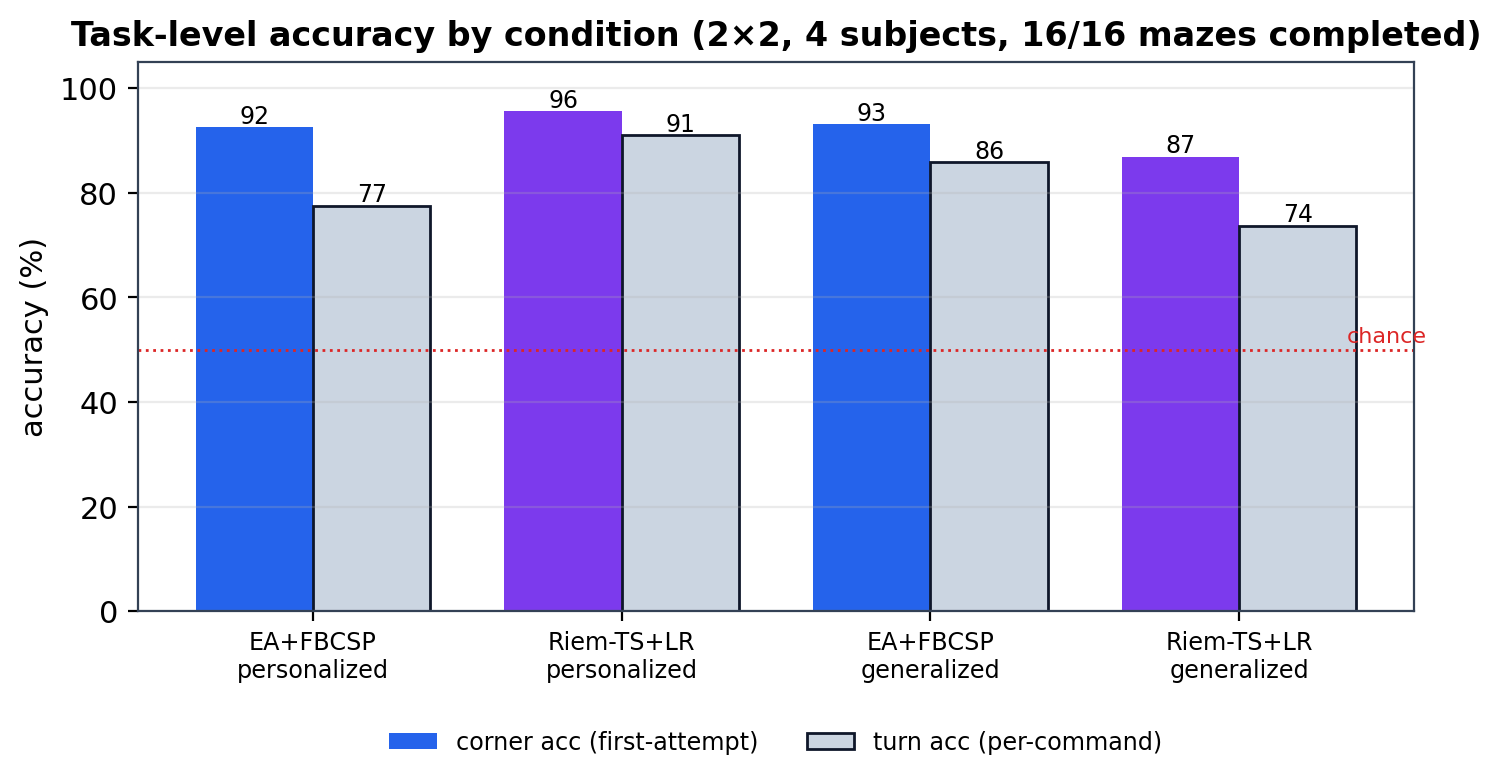
\includegraphics[width=\linewidth]{results_2x2.png}
  \caption{Task-level accuracy by condition. Corner accuracy (first-attempt, coloured)
  vastly exceeds chance; per-command turn accuracy (grey) is lower because it counts recovery
  commands. All 16 mazes were completed.}
  \label{fig:results}
\end{figure}

\begin{figure}[t]\centering
  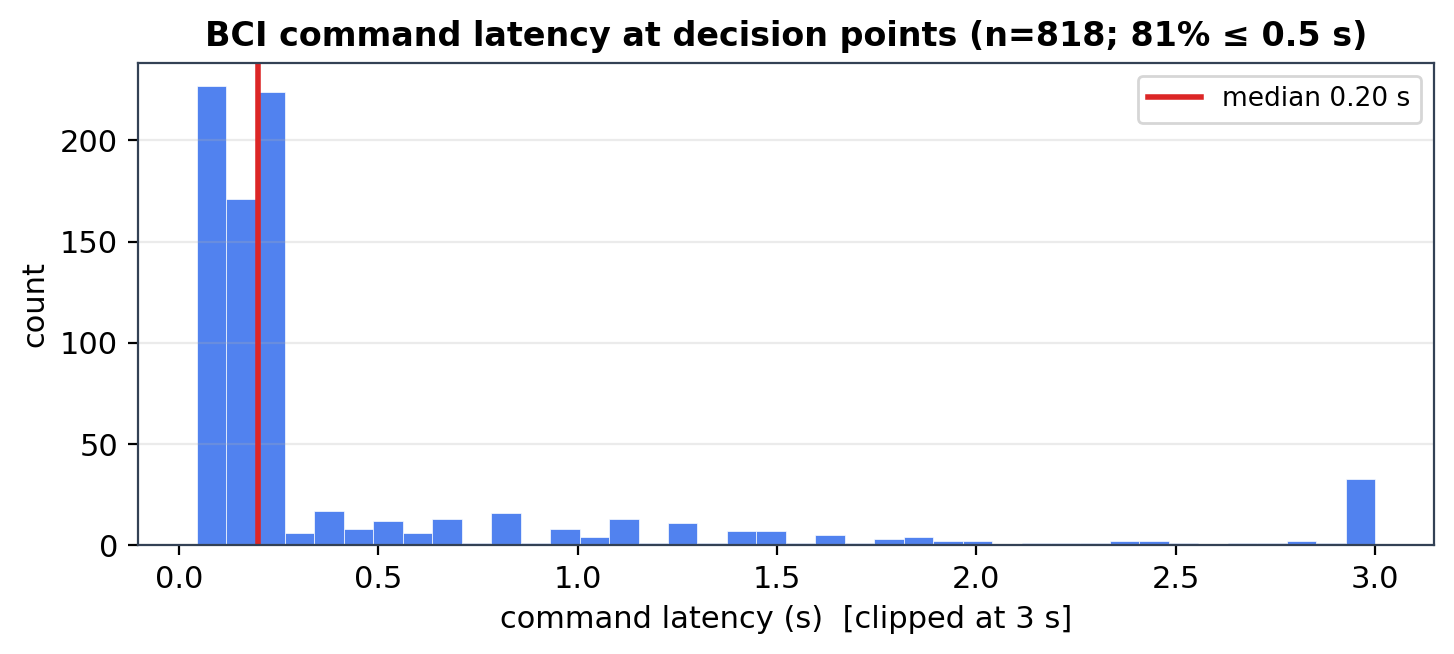
\includegraphics[width=\linewidth]{latency.png}
  \caption{Distribution of BCI command latency at decision points ($n{=}818$ commands);
  median 0.20\,s, 81\,\% within 0.5\,s.}
  \label{fig:latency}
\end{figure}

\begin{figure}[t]\centering
  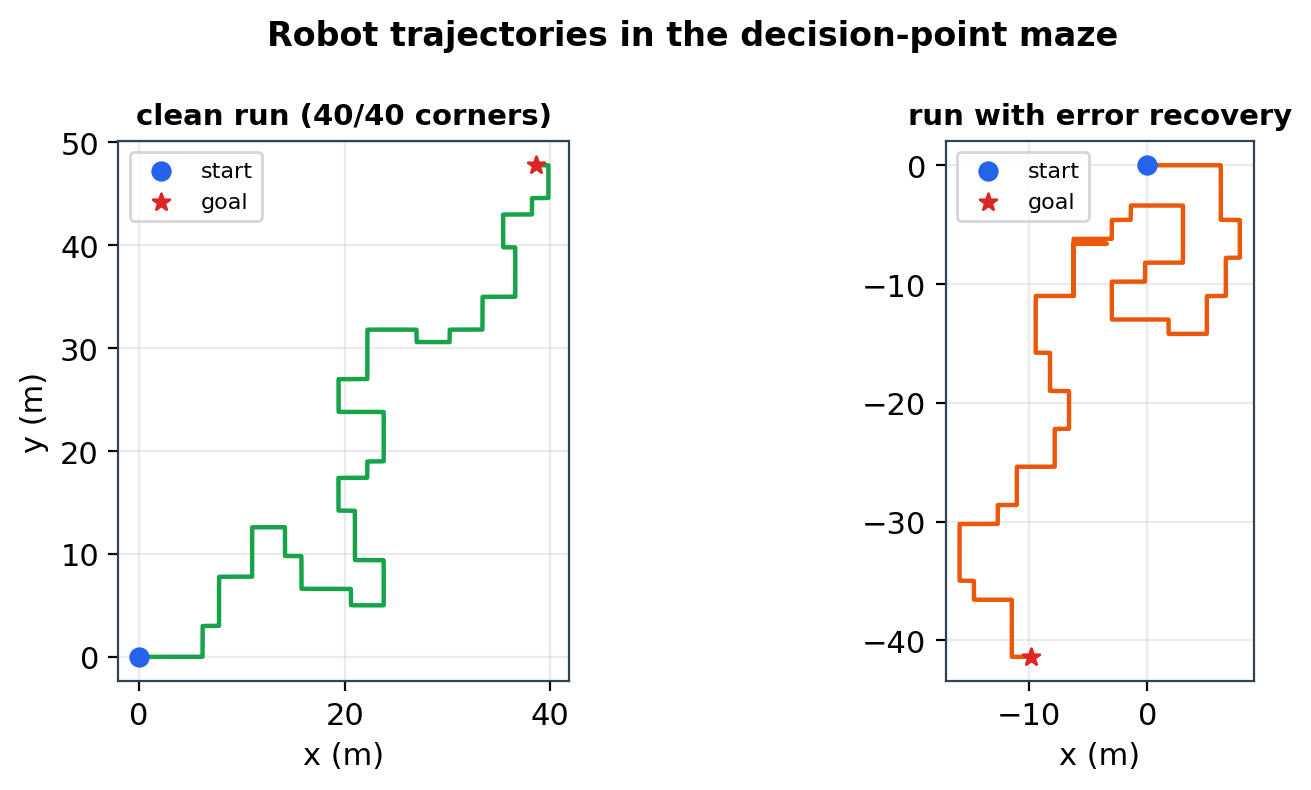
\includegraphics[width=\linewidth]{trajectory.png}
  \caption{Example robot trajectories: a clean run (left) and a run with an error-recovery
  loop (right); both reach the goal.}
  \label{fig:traj}
\end{figure}

\begin{figure}[t]\centering
  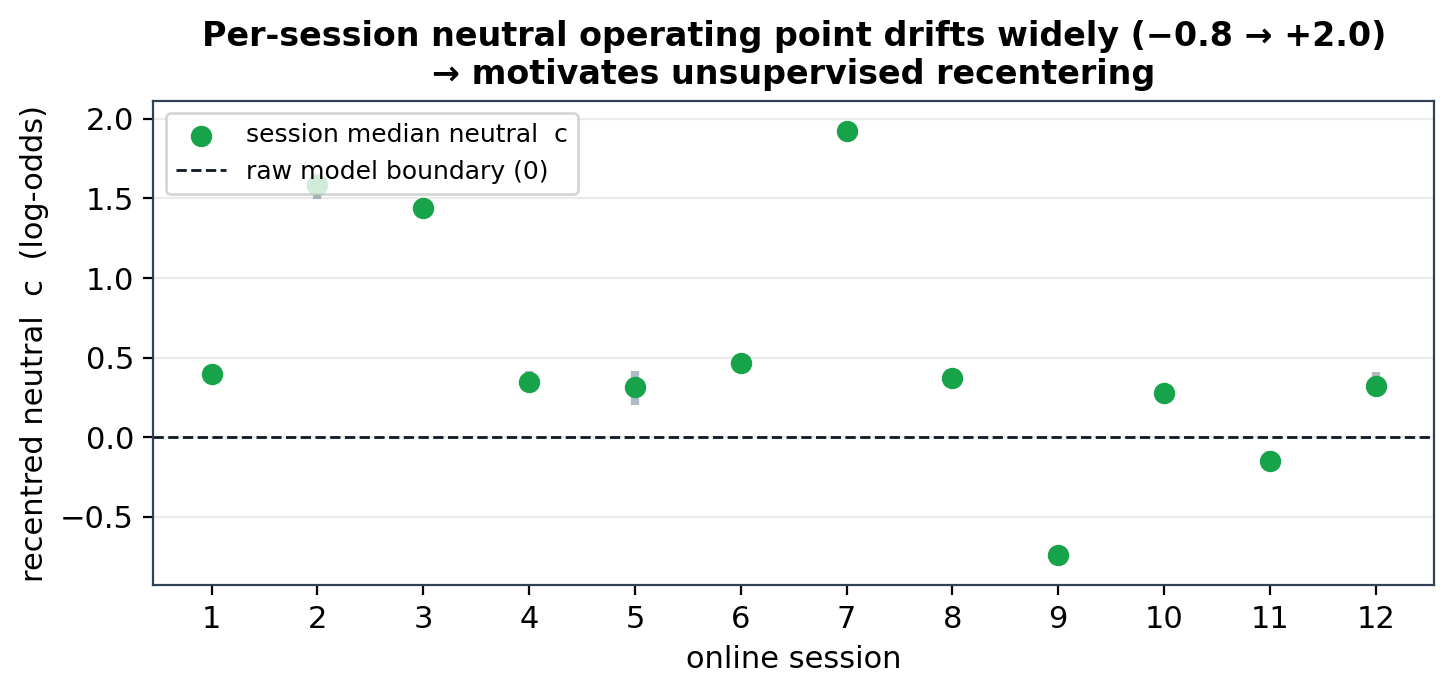
\includegraphics[width=\linewidth]{center_drift.png}
  \caption{The per-session neutral operating point $c$ varies widely across online sessions
  ($-0.8$ to $+2.0$ log-odds), motivating unsupervised recentering of a frozen decoder.}
  \label{fig:drift}
\end{figure}

% ============================================================ VIII. DISCUSSION
\section{Discussion}
Three findings stand out. First, \emph{decision-point shared control makes the BCI's job small
and its errors cheap}: one command per junction, a sub-second median latency, and local recovery
that turned $\sim$92\,\% per-corner decoding into full task completion. Second, \emph{a single
generalized model is competitive}: pooling users' data (including the driving user) matched
per-user models within a few points for EA+FB-CSP, suggesting that maintaining one shared decoder
rather than one per user is a viable deployment simplification---though, because the pool includes
the user, this is a shared-model result, not a zero-shot subject-independent one. Third,
\emph{the online neutral point genuinely drifts} across sessions (Fig.~\ref{fig:drift}), which a
fixed threshold cannot follow; the unsupervised recentering tracks it without labels or
retraining, consistent with the frozen-decoder design. The two decoder families were comparable
on average, with the Riemannian pipeline more sensitive to whether training was personalized.

% ============================================================ IX. LIMITATIONS
\section{Limitations}\label{sec:limits}
The evaluation is in a \emph{kinematic simulator} with limited autonomy (heading-hold and
range-based stopping; no dynamics, wall-following, or planning), so absolute times and the
control law would differ on hardware; physical-robot validation is the essential next step. The
in-the-loop study has four users and one trial per condition, which supports descriptive
comparison but not strong statistical inference; a larger cohort with repeated measures is needed.
The generalized condition includes the driving user's data, so we make no subject-independent
claim. Finally, the waiting state is unbounded (no timeout), and we did not isolate the
recentering component with an in-loop ablation---both are targeted in ongoing work.

% ============================================================ X. CONCLUSION
\section{Conclusion}
We presented a decision-point shared-control framework that lets a frozen, self-calibrating
MI-BCI drive robot navigation, keeping the decoder aligned to each session with unsupervised,
label-free recentering. In a $2{\times}2$ in-the-loop study, users completed every maze with
92\,\% per-corner accuracy and 0.20\,s median command latency, and a single generalized decoder
was competitive with per-user models. The results indicate that careful interaction design---asking
the BCI only at decision points and making errors recoverable---can yield reliable task-level
performance from imperfect EEG decoding. Physical-robot validation, a larger cohort, and an
in-loop ablation of the recentering component are the priorities for future work.

\bibliographystyle{IEEEtran}
\bibliography{refs}
\end{document}
